%10. Develop a LaTeX script to design a simple tree diagram or hierarchical structure in the 
%document with appropriate labels using the Tikz library Program:  

\documentclass{article}  
\usepackage{tikz} % Package for drawing diagrams  
\begin{document}  
\title{Simple Tree Diagram}  
\author{Hemanth S.P} % Replace with your name 
\date{\today} 
\maketitle 
\section*{Tree Diagram Example}  
Below is a simple hierarchical tree diagram created using the TikZ package: 
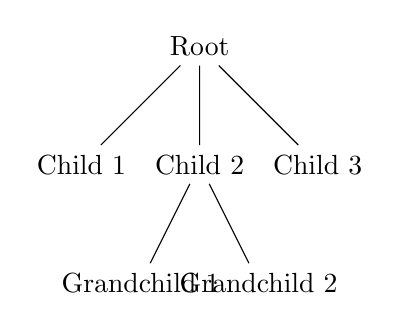
\begin{tikzpicture} % Start of the tree diagram 
% Define the main nodes (root node and its children) 
\node {Root} % Root node  
child {node {Child 1}} % First child of root 
child {node {Child 2} % Second  child of root  
child {node {Grandchild 1}} % Child of Child 2 
child {node {Grandchild 2}} % Another child of Child 2 
} 
child {node {Child 3}}; % Third child of root  
\end{tikzpicture} 
\end{document}